<<<<<<< HEAD
% GNUPLOT: LaTeX picture with Postscript
\begingroup
  \makeatletter
  \providecommand\color[2][]{%
    \GenericError{(gnuplot) \space\space\space\@spaces}{%
      Package color not loaded in conjunction with
      terminal option `colourtext'%
    }{See the gnuplot documentation for explanation.%
    }{Either use 'blacktext' in gnuplot or load the package
      color.sty in LaTeX.}%
    \renewcommand\color[2][]{}%
  }%
  \providecommand\includegraphics[2][]{%
    \GenericError{(gnuplot) \space\space\space\@spaces}{%
      Package graphicx or graphics not loaded%
    }{See the gnuplot documentation for explanation.%
    }{The gnuplot epslatex terminal needs graphicx.sty or graphics.sty.}%
    \renewcommand\includegraphics[2][]{}%
  }%
  \providecommand\rotatebox[2]{#2}%
  \@ifundefined{ifGPcolor}{%
    \newif\ifGPcolor
    \GPcolortrue
  }{}%
  \@ifundefined{ifGPblacktext}{%
    \newif\ifGPblacktext
    \GPblacktexttrue
  }{}%
  % define a \g@addto@macro without @ in the name:
  \let\gplgaddtomacro\g@addto@macro
  % define empty templates for all commands taking text:
  \gdef\gplbacktext{}%
  \gdef\gplfronttext{}%
  \makeatother
  \ifGPblacktext
    % no textcolor at all
    \def\colorrgb#1{}%
    \def\colorgray#1{}%
  \else
    % gray or color?
    \ifGPcolor
      \def\colorrgb#1{\color[rgb]{#1}}%
      \def\colorgray#1{\color[gray]{#1}}%
      \expandafter\def\csname LTw\endcsname{\color{white}}%
      \expandafter\def\csname LTb\endcsname{\color{black}}%
      \expandafter\def\csname LTa\endcsname{\color{black}}%
      \expandafter\def\csname LT0\endcsname{\color[rgb]{1,0,0}}%
      \expandafter\def\csname LT1\endcsname{\color[rgb]{0,1,0}}%
      \expandafter\def\csname LT2\endcsname{\color[rgb]{0,0,1}}%
      \expandafter\def\csname LT3\endcsname{\color[rgb]{1,0,1}}%
      \expandafter\def\csname LT4\endcsname{\color[rgb]{0,1,1}}%
      \expandafter\def\csname LT5\endcsname{\color[rgb]{1,1,0}}%
      \expandafter\def\csname LT6\endcsname{\color[rgb]{0,0,0}}%
      \expandafter\def\csname LT7\endcsname{\color[rgb]{1,0.3,0}}%
      \expandafter\def\csname LT8\endcsname{\color[rgb]{0.5,0.5,0.5}}%
    \else
      % gray
      \def\colorrgb#1{\color{black}}%
      \def\colorgray#1{\color[gray]{#1}}%
      \expandafter\def\csname LTw\endcsname{\color{white}}%
      \expandafter\def\csname LTb\endcsname{\color{black}}%
      \expandafter\def\csname LTa\endcsname{\color{black}}%
      \expandafter\def\csname LT0\endcsname{\color{black}}%
      \expandafter\def\csname LT1\endcsname{\color{black}}%
      \expandafter\def\csname LT2\endcsname{\color{black}}%
      \expandafter\def\csname LT3\endcsname{\color{black}}%
      \expandafter\def\csname LT4\endcsname{\color{black}}%
      \expandafter\def\csname LT5\endcsname{\color{black}}%
      \expandafter\def\csname LT6\endcsname{\color{black}}%
      \expandafter\def\csname LT7\endcsname{\color{black}}%
      \expandafter\def\csname LT8\endcsname{\color{black}}%
    \fi
  \fi
    \setlength{\unitlength}{0.0500bp}%
    \ifx\gptboxheight\undefined%
      \newlength{\gptboxheight}%
      \newlength{\gptboxwidth}%
      \newsavebox{\gptboxtext}%
    \fi%
    \setlength{\fboxrule}{0.5pt}%
    \setlength{\fboxsep}{1pt}%
    \definecolor{tbcol}{rgb}{1,1,1}%
\begin{picture}(7200.00,5040.00)%
    \gplgaddtomacro\gplbacktext{%
      \csname LTb\endcsname%%
      \put(1078,704){\makebox(0,0)[r]{\strut{}$0$}}%
      \csname LTb\endcsname%%
      \put(1078,1218){\makebox(0,0)[r]{\strut{}$5000$}}%
      \csname LTb\endcsname%%
      \put(1078,1733){\makebox(0,0)[r]{\strut{}$10000$}}%
      \csname LTb\endcsname%%
      \put(1078,2247){\makebox(0,0)[r]{\strut{}$15000$}}%
      \csname LTb\endcsname%%
      \put(1078,2762){\makebox(0,0)[r]{\strut{}$20000$}}%
      \csname LTb\endcsname%%
      \put(1078,3276){\makebox(0,0)[r]{\strut{}$25000$}}%
      \csname LTb\endcsname%%
      \put(1078,3790){\makebox(0,0)[r]{\strut{}$30000$}}%
      \csname LTb\endcsname%%
      \put(1078,4305){\makebox(0,0)[r]{\strut{}$35000$}}%
      \csname LTb\endcsname%%
      \put(1078,4819){\makebox(0,0)[r]{\strut{}$40000$}}%
      \csname LTb\endcsname%%
      \put(1210,484){\makebox(0,0){\strut{}$0$}}%
      \csname LTb\endcsname%%
      \put(1718,484){\makebox(0,0){\strut{}$10$}}%
      \csname LTb\endcsname%%
      \put(2227,484){\makebox(0,0){\strut{}$20$}}%
      \csname LTb\endcsname%%
      \put(2735,484){\makebox(0,0){\strut{}$30$}}%
      \csname LTb\endcsname%%
      \put(3244,484){\makebox(0,0){\strut{}$40$}}%
      \csname LTb\endcsname%%
      \put(3752,484){\makebox(0,0){\strut{}$50$}}%
      \csname LTb\endcsname%%
      \put(4261,484){\makebox(0,0){\strut{}$60$}}%
      \csname LTb\endcsname%%
      \put(4769,484){\makebox(0,0){\strut{}$70$}}%
      \csname LTb\endcsname%%
      \put(5278,484){\makebox(0,0){\strut{}$80$}}%
      \csname LTb\endcsname%%
      \put(5786,484){\makebox(0,0){\strut{}$90$}}%
      \csname LTb\endcsname%%
      \put(6295,484){\makebox(0,0){\strut{}$100$}}%
      \csname LTb\endcsname%%
      \put(6803,484){\makebox(0,0){\strut{}$110$}}%
      \put(1718,776){\makebox(0,0)[l]{\strut{}$\chi^2 = 909.47430$}}%
      \put(4769,776){\makebox(0,0)[l]{\strut{}$\sigma = 4.74793$}}%
    }%
    \gplgaddtomacro\gplfronttext{%
      \csname LTb\endcsname%%
      \put(2266,4646){\makebox(0,0)[r]{\strut{}files u 1:2}}%
      \csname LTb\endcsname%%
      \put(2266,4426){\makebox(0,0)[r]{\strut{}$f(x)$}}%
      \csname LTb\endcsname%%
      \put(209,2761){\rotatebox{-270.00}{\makebox(0,0){\strut{}events/\#}}}%
      \put(4006,154){\makebox(0,0){\strut{}position/mm}}%
    }%
    \gplbacktext
    \put(0,0){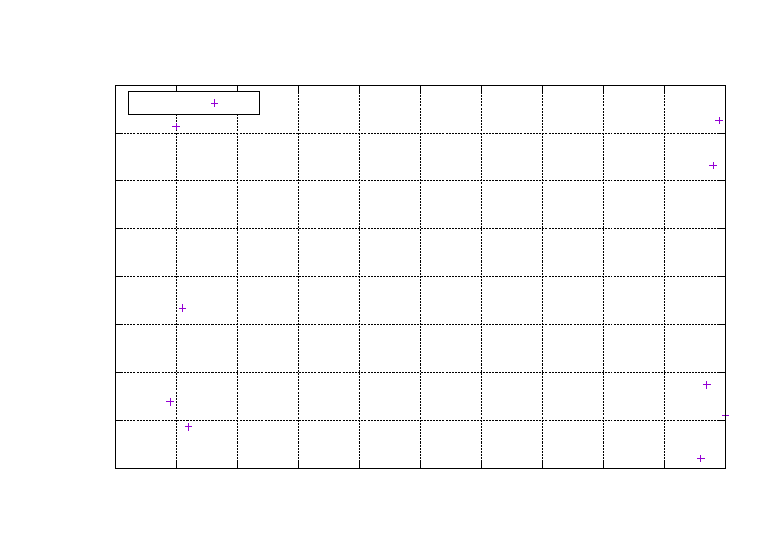
\includegraphics[width={360.00bp},height={252.00bp}]{output_1}}%
    \gplfronttext
  \end{picture}%
\endgroup
=======
>>>>>>> d750697aa22c5d5d154552b733b9e91d4ed7cf7c
